\begin{figure}[h]
  \centering
  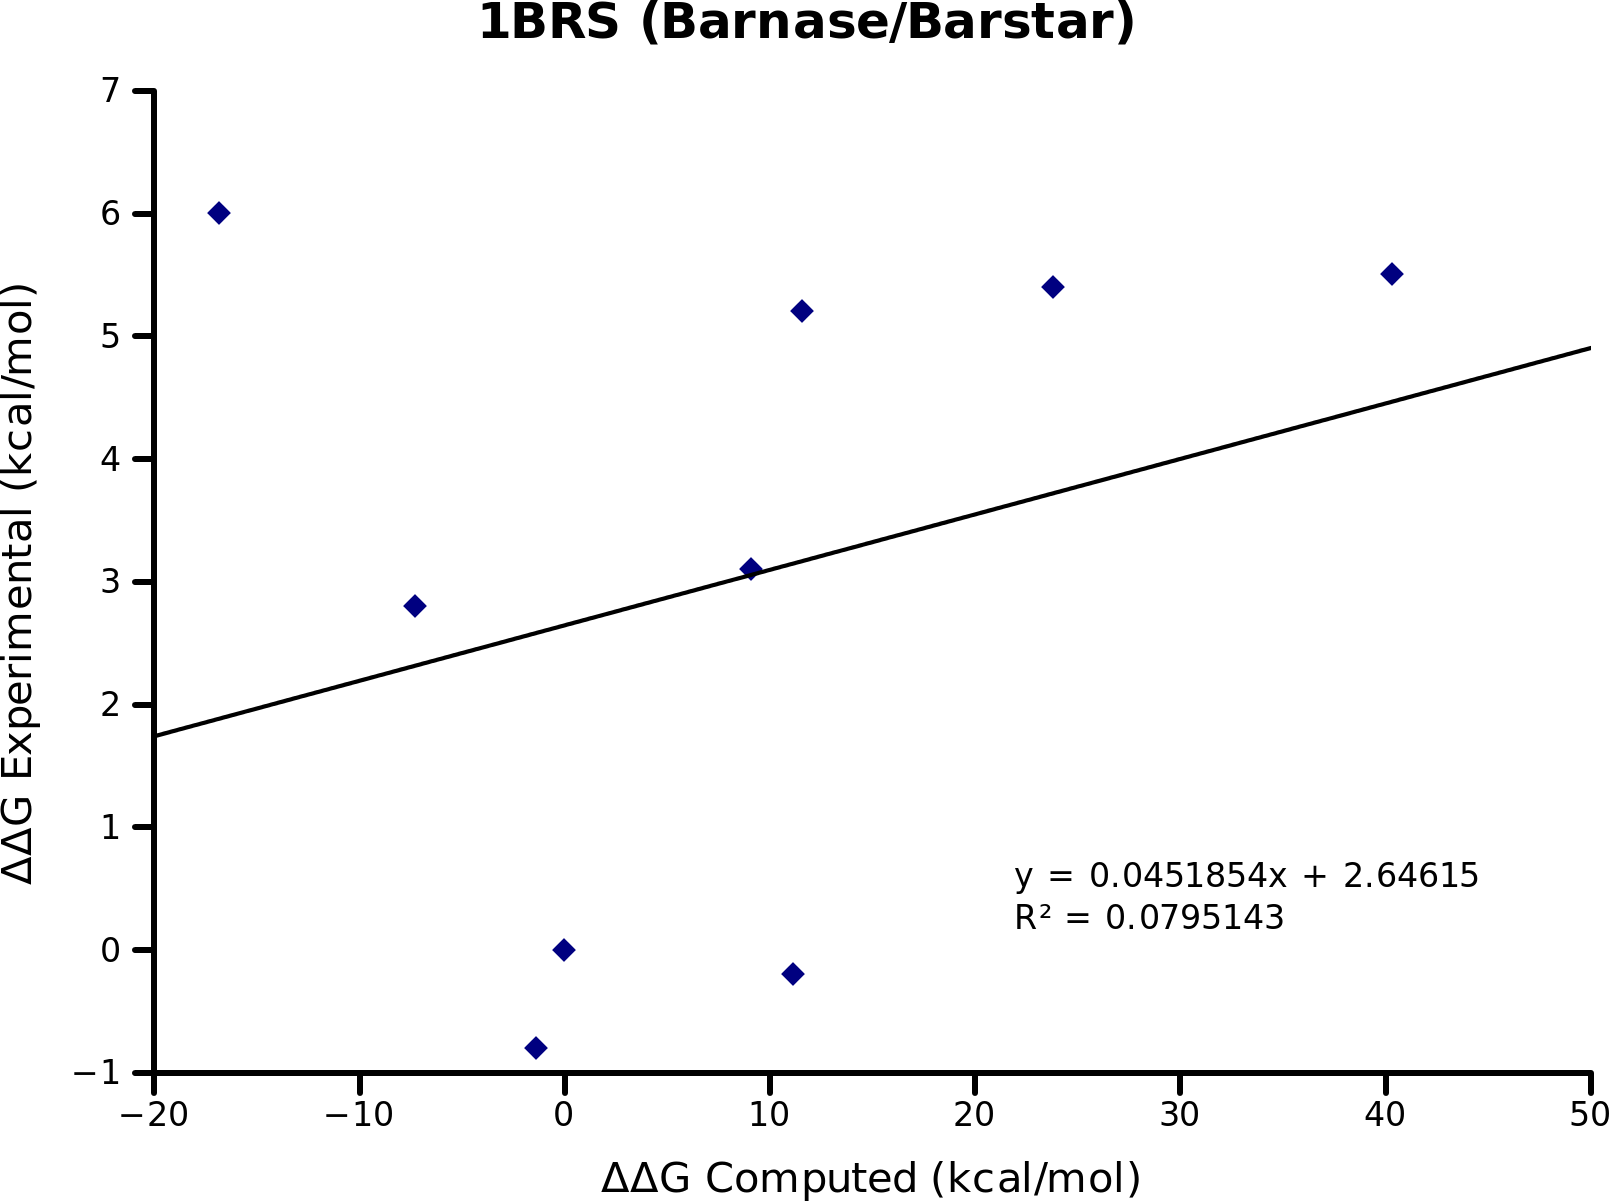
\includegraphics[width=0.65\textwidth]{figures/1brs_barnase_barstar.png}
  \caption{
Computed versus experimental \ddg\ binding for 8 alanine mutations in the Barstar-Barnase binding pair.
Crystal structure used for computations was 1BRS.
Specific amino acids mutated were residues 27, 54, 58, 59, 60, 73, 87, and 102, all of chain A.
Experimental binding affinity taken from \protect\cite{thorn2001asedb}.
            }
\end{figure}

\begin{figure}[h]
  \centering
  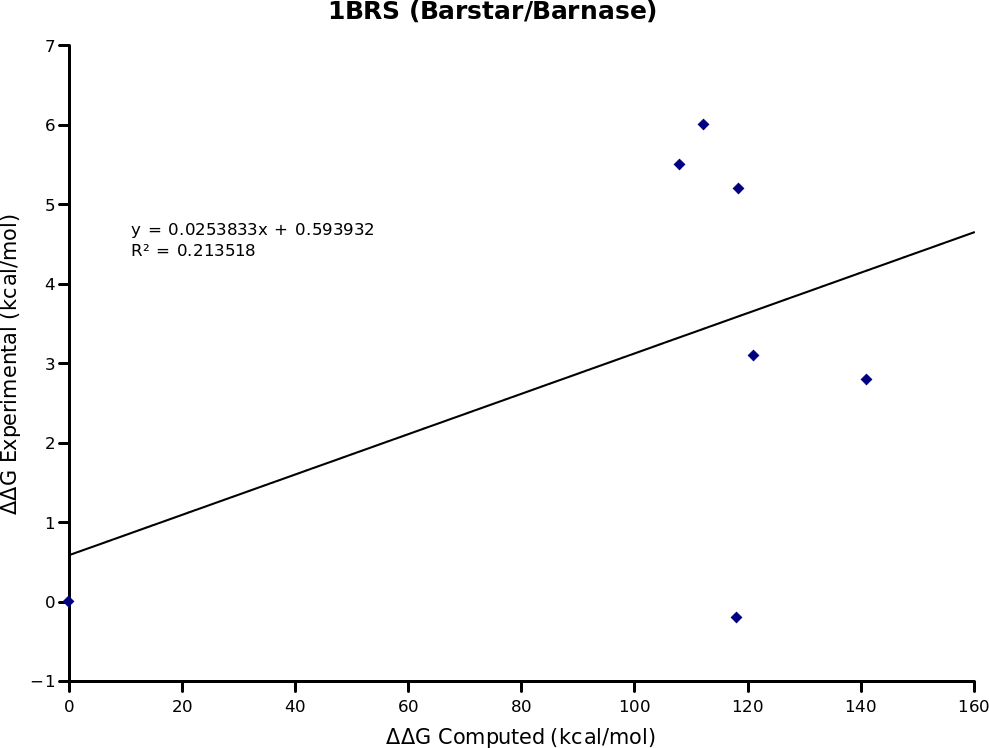
\includegraphics[width=0.65\textwidth]{figures/1brs_barstar_barnase.png}
  \caption{
Computed versus experimental \ddg\ binding for 6 alanine mutations in the Barstar-Barnase binding pair.
Crystal structure used for computations was 1BRS \protect\cite{buckle1994protein}.
Specific amino acids mutated were residues 29, 35, 39, 42, 74, and 78, all of chain D.
Experimental binding affinity taken from \protect\cite{thorn2001asedb}.
            }
\end{figure}

\begin{figure}[h]
    \centering
  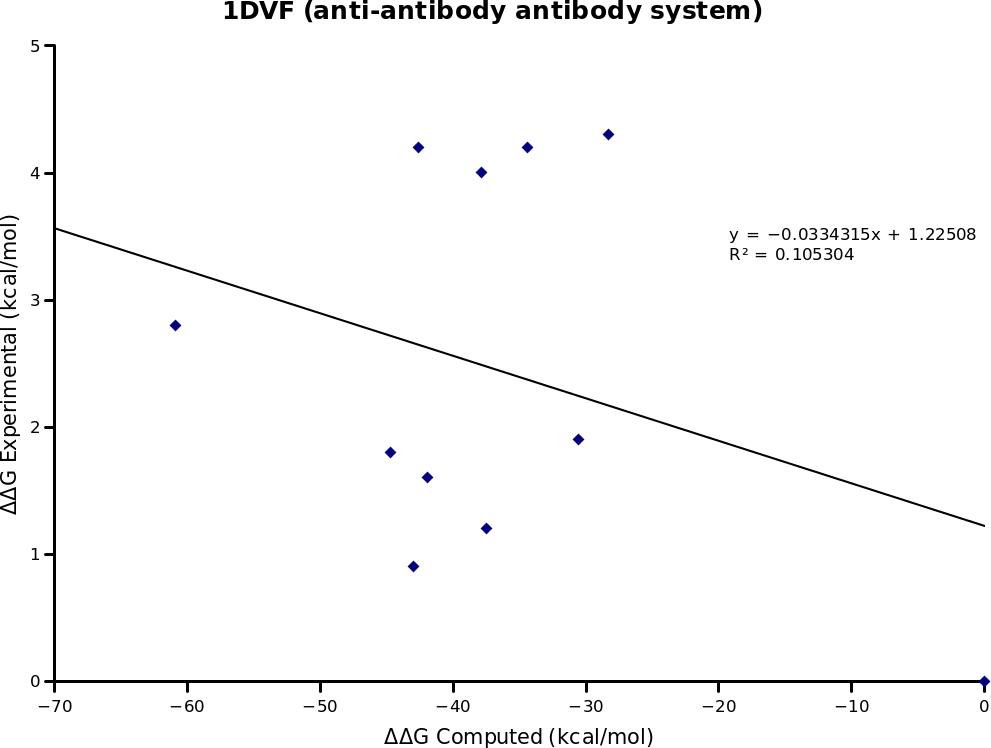
\includegraphics[width=0.65\textwidth]{figures/1dvf.png}
  \caption{
Computed versus experimental \ddg\ binding for 10 alanine mutations in the anti-hen-egg-white lysozyme antibody (D1.3) anti-idiotopic antibody (E5.2) complex.
Crystal structure used for computations was 1DVF \protect\cite{braden1996crystal}.
Specific amino acids mutated were residues 30, 32, 52, 54, 56, 58, 98, 99, 100, and 101, all of chain A.
Experimental binding affinity taken from \protect\cite{thorn2001asedb}.
            }
\end{figure}

\begin{figure}[h]
    \centering
  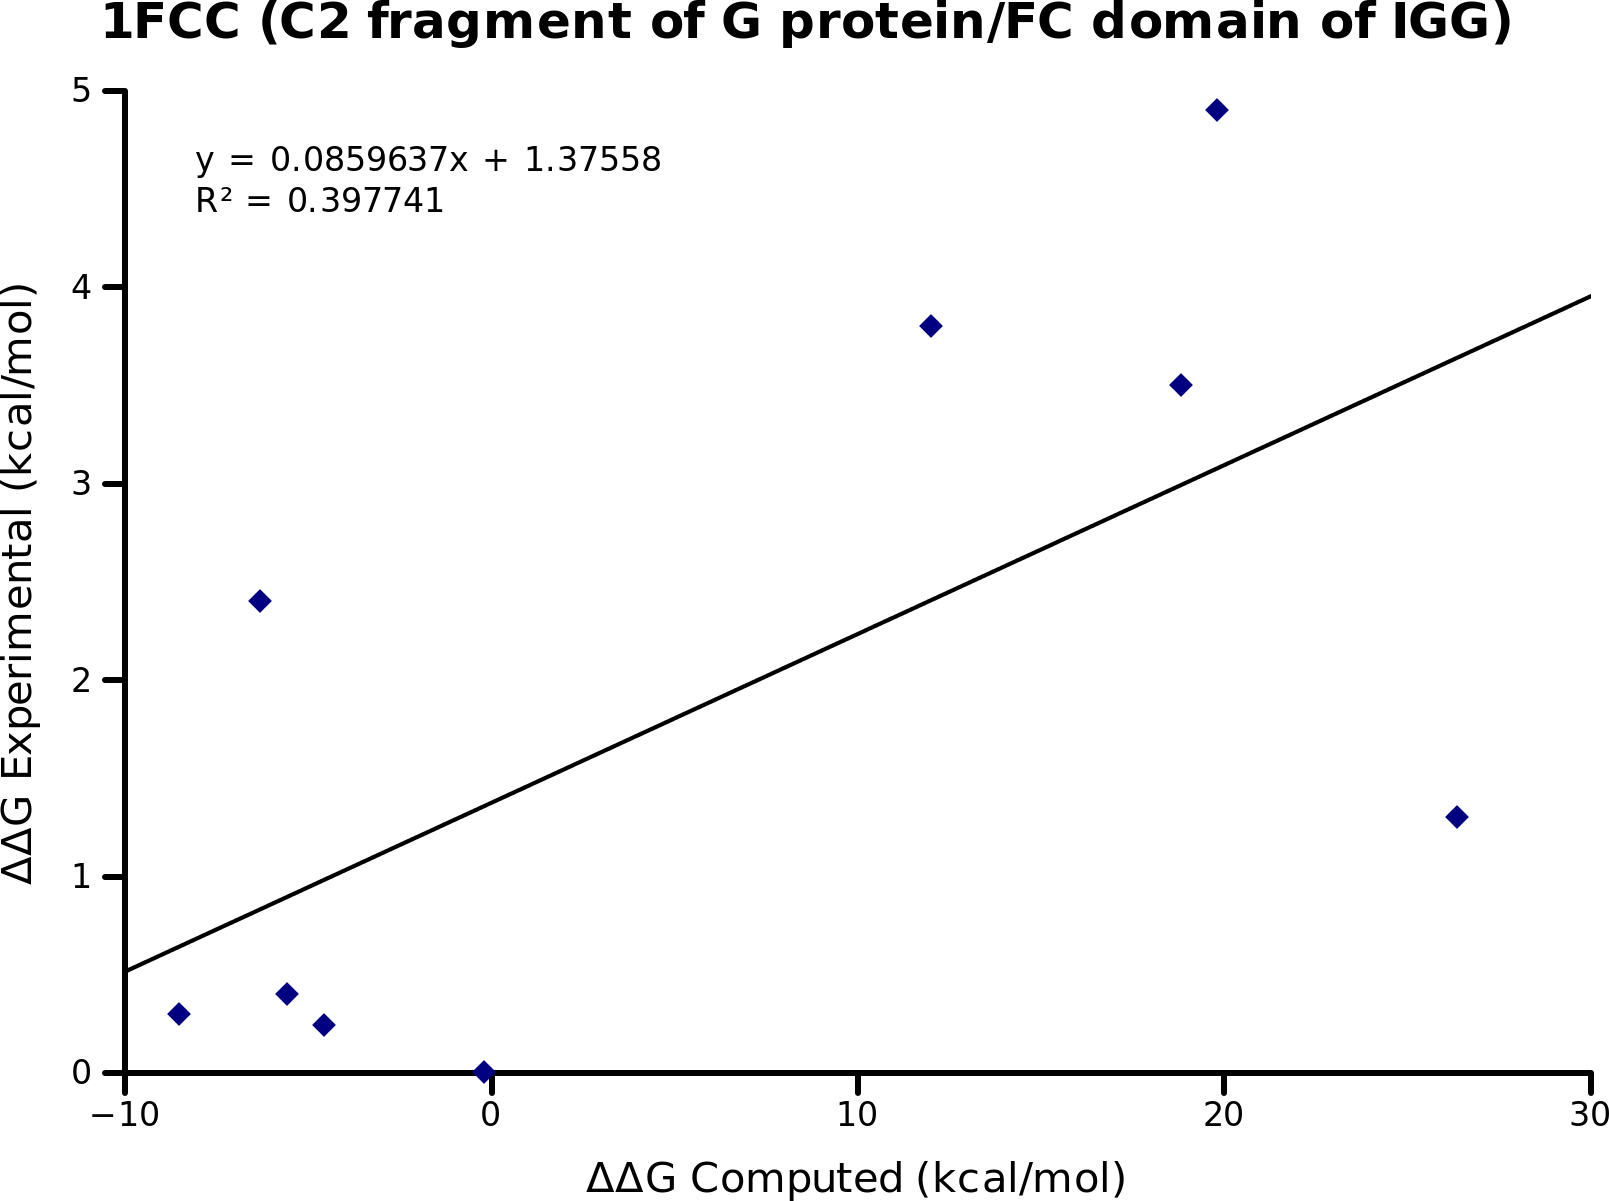
\includegraphics[width=0.65\textwidth]{figures/1fcc.png}
  \caption{
Computed versus experimental \ddg\ binding for 8 alanine mutations in  binding pair.
Crystal structure used for computations was 1FCC.
Specific amino acids mutated were residues 25, 27, 28, 31, 35, 40, 42, and 43, all of chain A.
Experimental binding affinity taken from \protect\cite{thorn2001asedb}.
            }
\end{figure}
